\documentclass[letterpaper]{article} % DO NOT CHANGE THIS
\usepackage[submission]{aaai2027} % DO NOT CHANGE THIS
\usepackage[hyphens]{url} % DO NOT CHANGE THIS
\usepackage{graphicx} % DO NOT CHANGE THIS
\graphicspath{{images/}}
\urlstyle{rm} % DO NOT CHANGE THIS
\def\UrlFont{\rm} % DO NOT CHANGE THIS
\usepackage{natbib} % DO NOT CHANGE THIS
\usepackage{caption} % DO NOT CHANGE THIS
\frenchspacing % DO NOT CHANGE THIS

\usepackage{amsmath}
\usepackage{amssymb}
\usepackage{booktabs}

\pdfinfo{
/TemplateVersion (2027.1)
}

\setcounter{secnumdepth}{0}
% Generated from confirmation V4 and V5 analyses; main_v3.tex is final.
% Do not edit empirical values by hand.
\newcommand{\VFourRegisteredBlocks}{60}
\newcommand{\VFourProviderConversations}{180}
\newcommand{\VFourRegisteredStrata}{18}
\newcommand{\VFourRealCandidateCount}{2}
\newcommand{\VFourRealAdmissions}{0}
\newcommand{\VFourCalibrationDecision}{Pass}
\newcommand{\VFourProviderTurns}{1379}
\newcommand{\VFourActions}{1379}
\newcommand{\VFourInputTokens}{2,249,799}
\newcommand{\VFourOutputTokens}{2,374,026}
\newcommand{\VFourTransportAttempts}{1,393}
\newcommand{\VFourPublicTestRequests}{226}
\newcommand{\VFourPublicTestPasses}{214}
\newcommand{\VFourPublicTestFailures}{12}
\newcommand{\VFourInvalidActions}{71}
\newcommand{\VFourExtraTransportAttempts}{14}
\newcommand{\VFourMinimumPassingCases}{61}
\newcommand{\VFourSubmittedRuns}{179}
\newcommand{\VFourPreregistrationDigest}{b5970f270d500fa526d478ba77774ab6095232f4573d092663efb9061d816fbb}
\newcommand{\VFourAnalyzerRepair}{Disclosed post-hoc compatibility audit}
\newcommand{\VFiveRegisteredBlocks}{18}
\newcommand{\VFiveProviderConversations}{54}
\newcommand{\VFiveNaturalCandidateCount}{1}
\newcommand{\VFiveNaturalAdmissions}{1}
\newcommand{\VFiveProviderTurns}{381}
\newcommand{\VFiveActions}{381}
\newcommand{\VFiveInputTokens}{562,563}
\newcommand{\VFiveOutputTokens}{520,587}
\newcommand{\VFiveTransportAttempts}{383}
\newcommand{\VFivePublicTestRequests}{65}
\newcommand{\VFivePublicTestPasses}{64}
\newcommand{\VFivePublicTestFailures}{1}
\newcommand{\VFiveInvalidActions}{17}
\newcommand{\VFiveExtraTransportAttempts}{2}
\newcommand{\VFiveSubmittedRuns}{54}
\newcommand{\VFivePreregistrationDigest}{6083729477053feeee328f79f9fddfcb83acdaae7410debdab5218b4e18e24eb}
\newcommand{\VFiveAnalysisDigest}{8b7849590c3a8080f7ed7c06eaea360c16833f0dfec62b855223740cf3e7879a}
\newcommand{\VFiveCrosscheckDigest}{02c6069c24ffd75f40e55db93597ac2ca89e345623f97f1017fd1997ea57f434}
\newcommand{\VFiveRawEvidenceDigest}{4845886b7cd14ee3e41b9988fb03b7a0a7d9da18adeffd63d232802545c94085}
\newcommand{\VFiveRawFileCount}{198}
\newcommand{\VFiveProviderResponseIDs}{381}
\newcommand{\AllRegisteredBlocks}{78}
\newcommand{\AllProviderConversations}{234}
\newcommand{\AllProviderTurns}{1760}
\newcommand{\AllActions}{1760}
\newcommand{\AllInputTokens}{2,812,362}
\newcommand{\AllOutputTokens}{2,894,613}
\newcommand{\AllTransportAttempts}{1,776}
\newcommand{\AllPublicTestRequests}{291}
\newcommand{\AllPublicTestPasses}{278}
\newcommand{\AllPublicTestFailures}{13}
\newcommand{\NonPlantedCandidateCount}{3}
\newcommand{\NonPlantedAdmissions}{1}
\newcommand{\SnapRealPublicTestFailures}{9}
\newcommand{\SnapRealBlocks}{18}
\newcommand{\SnapRealBSuccesses}{0}
\newcommand{\SnapRealBMeanScore}{0.000}
\newcommand{\SnapRealFSuccesses}{15}
\newcommand{\SnapRealFMeanScore}{0.877}
\newcommand{\SnapRealSSuccesses}{5}
\newcommand{\SnapRealSMeanScore}{0.321}
\newcommand{\SnapRealFullSliceGap}{10}
\newcommand{\SnapRealSuccessMatches}{6}
\newcommand{\SnapRealFullSuccessSliceFailure}{11}
\newcommand{\SnapRealFullFailureSliceSuccess}{1}
\newcommand{\SnapRealDecision}{Reject}
\newcommand{\ToolformerRealPublicTestFailures}{1}
\newcommand{\ToolformerRealBlocks}{18}
\newcommand{\ToolformerRealBSuccesses}{0}
\newcommand{\ToolformerRealBMeanScore}{0.000}
\newcommand{\ToolformerRealFSuccesses}{17}
\newcommand{\ToolformerRealFMeanScore}{0.944}
\newcommand{\ToolformerRealSSuccesses}{8}
\newcommand{\ToolformerRealSMeanScore}{0.481}
\newcommand{\ToolformerRealFullSliceGap}{9}
\newcommand{\ToolformerRealSuccessMatches}{9}
\newcommand{\ToolformerRealFullSuccessSliceFailure}{9}
\newcommand{\ToolformerRealFullFailureSliceSuccess}{0}
\newcommand{\ToolformerRealDecision}{Reject}
\newcommand{\PlantedPositivePublicTestFailures}{2}
\newcommand{\PlantedPositiveBlocks}{18}
\newcommand{\PlantedPositiveBSuccesses}{0}
\newcommand{\PlantedPositiveBMeanScore}{0.000}
\newcommand{\PlantedPositiveFSuccesses}{18}
\newcommand{\PlantedPositiveFMeanScore}{1.000}
\newcommand{\PlantedPositiveSSuccesses}{17}
\newcommand{\PlantedPositiveSMeanScore}{0.944}
\newcommand{\PlantedPositiveFullSliceGap}{1}
\newcommand{\PlantedPositiveSuccessMatches}{17}
\newcommand{\PlantedPositiveFullSuccessSliceFailure}{1}
\newcommand{\PlantedPositiveFullFailureSliceSuccess}{0}
\newcommand{\PlantedPositiveDecision}{Pass}
\newcommand{\IdentityControlPublicTestFailures}{0}
\newcommand{\IdentityControlBlocks}{6}
\newcommand{\IdentityControlBSuccesses}{0}
\newcommand{\IdentityControlBMeanScore}{0.000}
\newcommand{\IdentityControlFSuccesses}{6}
\newcommand{\IdentityControlFMeanScore}{1.000}
\newcommand{\IdentityControlSSuccesses}{5}
\newcommand{\IdentityControlSMeanScore}{0.833}
\newcommand{\IdentityControlFullSliceGap}{1}
\newcommand{\IdentityControlSuccessMatches}{5}
\newcommand{\IdentityControlFullSuccessSliceFailure}{1}
\newcommand{\IdentityControlFullFailureSliceSuccess}{0}
\newcommand{\IdentityControlDecision}{Pass}
\newcommand{\IdentityControlMatches}{5}
\newcommand{\IdentityControlSuccessGap}{1}
\newcommand{\ToolformerNaturalPublicTestFailures}{1}
\newcommand{\ToolformerNaturalBlocks}{18}
\newcommand{\ToolformerNaturalBSuccesses}{0}
\newcommand{\ToolformerNaturalBMeanScore}{0.000}
\newcommand{\ToolformerNaturalFSuccesses}{18}
\newcommand{\ToolformerNaturalFMeanScore}{1.000}
\newcommand{\ToolformerNaturalSSuccesses}{17}
\newcommand{\ToolformerNaturalSMeanScore}{0.944}
\newcommand{\ToolformerNaturalFullSliceGap}{1}
\newcommand{\ToolformerNaturalSuccessMatches}{17}
\newcommand{\ToolformerNaturalFullSuccessSliceFailure}{1}
\newcommand{\ToolformerNaturalFullFailureSliceSuccess}{0}
\newcommand{\ToolformerNaturalDecision}{Admit}


\title{EffectSlice: Evidence-Carrying Admission for Paper-Derived Procedural Cores}
\author{Anonymous Submission}
\affiliations{}

\begin{document}

\maketitle

\begin{abstract}
Turning a paper into a compact agent artifact does not make that artifact a
reliable substitute: source provenance and behavioral sufficiency are different
claims.  We introduce \textbf{EffectSlice}, a proof-of-concept, reducer-agnostic
candidate-admission protocol and evidence package
for paper-derived procedural cores.  Given a no-artifact baseline (B), registered
full artifact (F), and selected strict subset (S), it binds instructions to paper
spans and dependencies, freezes the candidate, permits visible public testing,
and scores each fresh terminal run once with a private suite.  Admission is a
hash-bound finite-schedule decision, not a population estimate.  Across two
sequentially registered schedules and \AllProviderConversations{} fresh DeepSeek
endpoint conversations, the protocol separates three decision states: SNAP
prefix 03 has insufficient F and S (0/15/5 B/F/S successes, Reject); Toolformer
prefix 01 has sufficient F but insufficient S (0/17/8, Reject); in a separately
registered later schedule, a local admission is issued for pre-existing
Toolformer prefix 04 (0/18/17, Admit) on a new nonoverlapping private registry.
A planted redundancy smoke test and byte-identical identity instrument pass
their registered internal checks.  These task-local outcomes do not establish
broad automatic reduction, paper-level equivalence, or human benefit.
\end{abstract}

\section{Introduction}

Paper-reproduction agents increasingly turn research descriptions into code and
executed experiments \cite{starace2025paperbench,zhao2025autoreproduce}, while
paper-to-agent systems package papers and associated software as interactive
tools \cite{miao2025paper2agent}.  Agent-skill systems likewise compile external
resources into reusable instructions
\cite{shen2026skillfoundry,pan2026anything2skill}.  Both can pair vendor inference
with local execution.

The difficult step is deciding what the reusable \emph{core} is.  A paper may
describe a five-step mechanism, while a reducer retains only the first three
steps because they were sufficient on one development example.  The resulting
artifact can be short and traceable to the paper without being a reliable
substitute for the complete procedure.  Conversely, a complete artifact can be
correct but inconsistently used by a bounded agent.  These are behavioral
questions that token counts and source overlap do not answer.

Recent work makes this tension concrete.  SkillReducer reports that large-scale
skill compression can improve functional quality
\cite{gao2026skillreducer}.  A controlled 1,200-rollout decomposition instead
finds no representation strategy that improves over raw skills and identifies
executor capability as the dominant factor \cite{xu2026compression}.  Both are
important optimization studies.  Our question is downstream and
candidate-specific: after any system proposes a paper-derived core, what evidence
is required before a user is told that it can stand in for the complete
paper-derived artifact?

Three requirements follow: source-addressed instructions and dependencies;
public feedback separated from terminal private scoring; and registered positive,
negative, and byte-identical controls.  Provenance establishes identity, not a
complete interpretation, while controls expose obvious gate or session failures.

We introduce \textbf{EffectSlice}, an evidence-carrying admission protocol rather
than a new compression algorithm.  It represents a paper-derived procedure as
source-addressed atoms, freezes a dependency-closed strict subset, and runs three
conditions: no artifact (B), the full artifact (F), and the selected slice (S).
Each condition receives a fresh provider conversation.  The public test is
visible and callable; the private 64-case scorer is invoked only on the fixed
terminal patch and its result is not returned for another model turn.  Separate
pre-run and post-run manifests bind the task, paper source, atoms, artifacts,
tests, scorer, runner, transport, schedule, outputs, and analysis lineage by
digest.

The evidence addresses three questions: whether realized B/F/S runs distinguish
full-artifact insufficiency from subset-only insufficiency (RQ1); whether positive,
negative, and identity controls exercise admission, rejection, and session-noise
sanity states (RQ2); and whether a post-selected candidate can earn a valid local
admission on a separately registered, nonoverlapping boundary (RQ3).

Our contributions are:
\begin{itemize}
    \item We operationalize a source-addressed atom schema with exact source
    locations, executable roles, dependency edges, and immutable artifact
    identities, separating provenance from behavioral sufficiency.
    \item Our main contribution is the candidate-level admission record:
    candidate and source
    identities, public/private information boundary, frozen schedule, immutable
    outcomes, and a binary finite-schedule Admit/Reject decision.  Reject means
    only ``do not admit under this registered boundary,'' and makes no IID,
    cross-paper, or population claim.
    \item Our proof of concept runs three non-planted prefix candidates plus
    positive, negative, and identity checks in two hash-registered schedules.
    V4 exposes full-artifact and subset-only insufficiency; fresh V5 evidence admits
    a pre-existing four-of-five-atom candidate.  The package preserves all
    \AllProviderConversations{} conversations, patches, scores, and digests, and
    cross-checks two disclosed analyzer compatibility repairs.
\end{itemize}

We do not claim a general compression advantage, lower cost, local-model
inference, full-paper reproduction, or benefit to human users.

\section{Related Work}

\paragraph{Paper reproduction and executable research.}
PaperBench evaluates agents that recreate AI research repositories
\cite{starace2025paperbench}; AutoReproduce adds paper lineage to automated
experiment reproduction \cite{zhao2025autoreproduce}; and Paper2Agent builds
interactive agents around papers and code, emphasizing reliable construction,
iterative testing, and source linkage \cite{miao2025paper2agent}.  We treat
Paper2Agent as an upstream full-agent generator: EffectSlice starts after a
registered full artifact exists and audits a later strict-subset substitution claim.

\paragraph{Skill construction, retrieval, and compression.}
SkillFoundry and Anything2Skill compile reusable skills from heterogeneous
sources \cite{shen2026skillfoundry,pan2026anything2skill}.  SkillReducer compresses
routing descriptions and skill bodies, then restores content when task feedback
shows a regression; it also reports an independent deterministic benchmark
\cite{gao2026skillreducer}.  Xu and Wu freeze ten skill-delivery conditions over
40 software tasks, compare raw, shortened, structured, and scoped forms, and use
task-clustered inference and real-cost accounting \cite{xu2026compression}.
Shaposhnikov et al. provide our strongest utility baseline by comparing behavior
with and without whole skills \cite{shaposhnikov2026agenticskills}.  Their Agentic
Skills Framework measures whole-skill marginal utility; our contrast fixes a strict
subset against a registered full-artifact adequacy control and binds the resulting
release identity to source locators and the evaluation boundary.
EffectSlice neither competes with their reducers nor repeats their cost question.
It adds source-span binding and a candidate-level admission record after the
candidate is frozen.

\begin{table*}[t]
\centering
\small
\setlength{\tabcolsep}{4pt}
\begin{tabular}{p{0.15\textwidth}p{0.24\textwidth}p{0.27\textwidth}p{0.25\textwidth}}
\toprule
Study & Artifact and objective & Evaluation boundary & Distinguishing output \\
\midrule
SkillReducer \cite{gao2026skillreducer} & Generic agent skills; token-efficient
routing and progressive disclosure & Self-correcting task feedback plus an
independent deterministic skill benchmark & Optimized skill and aggregate
retention/quality \\
Xu and Wu \cite{xu2026compression} & Raw and transformed skills; quality/cost
factor decomposition & 40 tasks, 10 conditions, three repetitions; task-clustered
contrasts & Multi-task aggregate condition comparison and cost diagnosis \\
Agentic Skills Framework \cite{shaposhnikov2026agenticskills} & Whole executable
skills; marginal utility & Scalable with-skill versus without-skill task
evaluation & Whole-skill utility across task/model configurations \\
EffectSlice (ours) & Source-addressed atoms from each source paper; admit or reject one
fixed strict subset & Visible public test, one terminal private score per fresh condition run, complete
registered finite schedule & Hash-bound candidate record with a task-local
admission or rejection \\
\bottomrule
\end{tabular}
\caption{Closest-work comparison.  EffectSlice is a downstream admission and
audit layer, not a claim of superior compression or broader empirical coverage.}
\label{tab:closest}
\end{table*}

The established components are reduction, holdout isolation, skill-utility
measurement, provenance, and digest manifests.  Our specific technical increment is
their coupling into a candidate-specific substitution decision and release record.
Despite its name, EffectSlice is an admission protocol, not a slicing algorithm.

\paragraph{Reduction and adaptive evaluation.}
Delta debugging and C-Reduce remove components while preserving observed behavior
\cite{regehr2012creduce}; prompt compression trades context size against retained
information \cite{jiang2023llmlingua}.  Repeated holdout exposure can overfit an
adaptively selected hypothesis \cite{dwork2015reusableholdout}.  EffectSlice applies
this information-flow lesson to tool-using code agents: public tests support
development, while the fixed patch receives one terminal private evaluation.  The
increment is binding that isolation to paper-source addresses, B/F/S candidate
identities, and an archival local decision record.

\section{Problem Setting}

Let paper $P$ have a cryptographic identity $d_P$.  We represent a bounded
paper-specific procedure as atoms $A=\{a_1,\ldots,a_K\}$ and a directed acyclic
dependency graph $G$.  Each atom stores
\begin{equation}
a_i=(\mathrm{id}_i,\ell_i,s_i,r_i,D_i),
\end{equation}
where $\ell_i$ is an exact source locator (document digest, byte and line spans),
$s_i$ is the executable instruction, $r_i$ its contract role, and $D_i$ the set
of atom IDs of its direct dependencies.  A candidate atom set
$A_S\subsetneq A$ is nonempty and dependency closed iff
$D_i\subseteq\{\mathrm{id}_j:a_j\in A_S\}$ for every $a_i\in A_S$.  A deterministic
renderer $R$, using topological order with atom-ID tie breaking, produces the
full artifact $F=R(A)$ and candidate artifact $S=R(A_S)$.  Both are registered
before confirmation.  This representation records provenance; it does not assert
semantic completeness or that an agent will use the instructions.

For registered block $r$, condition $C\in\{B,F,S\}$ starts a fresh conversation
with the same task, an isolated copy of the same starter workspace, action
interface, public test, action budget, and private scorer.  Only the artifact
context differs.  Let $q_{C,r}\in[0,1]$ be the terminal private score,
$t_{C,r}$ indicate the hard task contract, and $p_{C,r}$ indicate that the
terminal patch was applied.  Operational success is
\begin{equation}
z_{C,r}=\mathbb{1}[t_{C,r}=1\land p_{C,r}=1\land q_{C,r}\geq 0.95].
\end{equation}
A threshold of 0.95 over 64 deterministic cases requires at least
\VFourMinimumPassingCases{}/64 cases.
The raw scorer's \texttt{success} flag means exact 64/64 success; every success
count in our tables and decisions instead uses the operational definition above.
Candidate rows use \emph{Admit/Reject}; control and integrity checks use
\emph{Pass/Fail}.  Provider or transport exhaustion, scorer failure, an empty
submission, or a missing or malformed registered output makes the schedule
Invalid/No record and supplies neither admission nor rejection evidence.  When a
valid scorer result exists but the terminal patch was not applied or the hard
contract fails, $z_{C,r}=0$ and the run remains in the registered denominator.

EffectSlice makes a finite engineering decision.  For an 18-block family, let
$k_C=\sum_r z_{C,r}$.  The candidate is admitted exactly when
\begin{equation}
\begin{split}
&k_B\leq 2,\quad k_F\geq 16,\quad k_S\geq 16,\\
&k_F-k_S\leq 2,
\end{split}
\label{eq:sla}
\end{equation}
and every registered output and schedule-level integrity check is complete.  Equation
\ref{eq:sla} is a Git-committed, hash-anchored service-level rule for this schedule.
For a complete valid schedule that misses this gate, the record says Reject: it
withholds admission under this frozen boundary rather than asserting that the
candidate is semantically invalid.  The binary decision applies only after the
completeness and integrity gate; malformed schedules produce no decision record.
It is not a confidence interval, prevalence estimate, or hypothesis about a
population of papers or provider sessions.

The four numeric fields use a uniform two-run tolerance chosen from prior
development evidence and frozen before V4; they are deployment parameters, not
universal constants or values fitted to V4 outcomes.  At $n=18$, the registered
$k_F-k_S\leq2$ field is logically implied by $k_S\geq16$ and $k_F\leq18$.  We
retain it because it was preregistered, but do not count it as independent
evidence.  Admission is therefore a count-level SLA, not block-level behavioral
equivalence.

The evidence-carrying output is a record
\begin{equation}
\mathcal{E}=(d_{\mathrm{pre}},M_{\mathrm{post}},\sigma,\mathcal{O},\delta),
\end{equation}
where the pre-run commitment root $d_{\mathrm{pre}}$ recursively binds $d_P$,
the atom map and graph, rendered artifacts, task, public and private tests,
scorer, bound analyzer, runner, transport, schedule $\sigma$, and their own
digests.  After execution, the digest-indexed archival manifest $M_{\mathrm{post}}$ binds
$d_{\mathrm{pre}}$, immutable output set $\mathcal{O}$, raw-evidence digest,
analysis and compatibility code, independent crosscheck, generated result
macros, and local decision $\delta$.  The supplied
\texttt{effectslice-paper-results-manifest.v5} file
\texttt{generated\_results\_manifest\_v5.json} is canonical; older numbered
manifests are superseded.  It preserves lineage but does not
retroactively preregister post-run repairs or derived artifacts.  A score
without these candidate, commitment, and information-boundary identities is not
an EffectSlice admission record.

\section{EffectSlice}

\subsection{Source-Addressed Candidate Construction}

The extraction stage creates the atom registry from quoted paper passages and
records dependencies separately from prose order.  A reducer may be heuristic,
learned, or interactive; the admission protocol only requires a deterministic
candidate identity and closure audit.  SNAP prefix 03 and Toolformer prefix 01
were locked before V4 provider calls.  Toolformer prefix 04 already existed in
the same deterministic reducer registry, but we selected it after inspecting V4,
then froze it before V5.  This project-local ordered prefix reducer is neither
our contribution nor an implementation of SkillReducer.

The closure auditor rejects unknown atom IDs, graph cycles, a non-strict set, or
any retained atom whose transitive prerequisite is absent.  It then renders with
the registered topological tie break and verifies $d_F$ and $d_S$.  Every V4 and
V5 strict-subset family passed these checks before its provider execution.  The atom
boundaries and dependency edges were author-engineered from the cited passages;
their semantic correctness was not independently adjudicated.

Table~\ref{tab:atoms} exposes the complete atom-ID inventory.  The SNAP candidate
retains preprocessing and degree construction but omits the linear-operator and
eigensolver/guard atoms.  Toolformer prefix 01 retains only the future-token
weight schedule; prefix 04 retains the loss, counterfactual, and threshold but
omits the all-candidate/order unit.  They are concrete core hypotheses.  Prefix
04 was selected using V4 results, so its claim rests only on the subsequently
registered V5 block, not on prospective V4 selection.

\begin{table*}[t]
\centering
\small
\begin{tabular}{p{0.14\textwidth}p{0.59\textwidth}p{0.18\textwidth}}
\toprule
Task/family & Registered source-addressed units in $F$ & Fixed $S$ \\
\midrule
SNAP-MFSE & A01 IDF scaling; A02 row normalization; A03 self-similarity removal
and degree; A04 matrix-free linear operator; A05 eigensolver, ordering, and
no-materialization guard.  \emph{Source/deps: extracted lines 73--79;
A01$\prec$A02$\prec$A03$\prec$A04$\prec$A05.} & A01--A03 (3/5) \\
Toolformer prefix 01 & T01 normalized future-token weights; T02 weighted loss; T03
stronger counterfactual; T04 inclusive threshold; T05 all-candidate/order rule.
\emph{Source/deps: lines 76--79, 134--171, 268--272;
T01$\prec$T02$\prec$T03$\prec$T04$\prec$T05.} & T01 (1/5) \\
Toolformer prefix 04 & T01--T05 and source/dependency chain as above.  This
candidate was a pre-existing output of the registered deterministic prefix
reducer. & T01--T04 (4/5) \\
Planted positive & T01--T05 above plus T06, a registered restatement of the
T04/T05 invariant that adds no computation.  \emph{T06 cites lines 76--79 and
159--171 and requires T04/T05.} & T01--T05 (5/6) \\
\bottomrule
\end{tabular}
\caption{Complete atom-ID inventory and explicit candidate boundary.  The bound
registry retains each atom's full locator, instruction, role, and dependency
fields, plus byte spans and file
digests.  The identity family uses
byte-identical $F$ and $S$ and is instrumentation, not a strict-subset candidate.}
\label{tab:atoms}
\end{table*}

\subsection{Public Development, Terminal Private Scoring}

The model sees the task, common action protocol, assigned artifact, an isolated
starter-workspace copy, and the public test file.  Within a 16-action budget it
may search, open, edit,
and run the public test.  Public output is returned and may guide another model
turn.  A \texttt{submit} action freezes the patch, invokes the private 64-case
scorer once, stores the result, and terminates the conversation.  If the action
budget ends with a nonempty patch, that final patch is scored once; an empty patch
fails without feedback.  No private result is sent back to the model.

The family manifest binds the paper text, atom map, $F$, $S$, public test,
private case registry, scorer, starter workspace, prompt, runner, analyzer,
transport, thresholds, block identifiers, and B/F/S order by SHA-256.  Output
directories are write-once.  Provider response IDs must be unique, and every
transport attempt is retained.  This yields a trace from a paper span to the
artifact seen by the model, its tool trajectory, the fixed patch, and the final
score.

\subsection{Controls and Interleaved Schedule}

V4 uses 18 temporal strata and at most two workers.  Every stratum contains SNAP,
Toolformer prefix 01 (also the negative control), and the planted positive; six
also contain identity instrumentation.  Each 18-block family balances all six
B/F/S orders three times, while identity uses each once: \VFourRegisteredBlocks{}
blocks and \VFourProviderConversations{} fresh conversations in total.

After V4, we selected pre-existing prefix 04.  V5 separately freezes 18 balanced
blocks and \VFiveProviderConversations{} fresh conversations over cases disjoint
from all earlier private cases by ID, seed, and payload digest.  It is new evidence
for a post-V4 candidate, not an extension of the V4 preregistration.

The planted family is a pipeline smoke test, not evidence of useful compression
or naturally redundant paper text.  The registered internal checks pass only if it is admitted,
the real negative
is rejected, identity instrumentation passes, all outputs exist, and integrity
holds.  Identity passes when at least five of six F/S success indicators match
and the aggregate F/S success-count gap is at most one.  At six pairs the latter
is implied by the former and is retained as a registered consistency field, not
independent evidence.  Identity does not require
the two fresh sessions to return the same patch or score.

\section{Experimental Setup}

\paragraph{Paper-specific tasks.}
SNAP-MFSE isolates SnapATAC2's matrix-free spectral embedding core
\cite{zhang2024snapatac2}: IDF scaling, row normalization, self-similarity
removal, degree construction, normalized operator application, and leading
spectral coordinates.  Toolformer filtering isolates the rule for retaining API
calls \cite{schick2023toolformer}: future-token weights, weighted losses, the
stronger counterfactual, inclusive thresholding, and ordered application to all
proposals.  Each V4 or V5 private block contains 64 deterministic cases and hard
interface/guard checks.  Cases characterize one terminal patch and are not
treated as independent model runs.

\paragraph{Freeze and holdout chronology.}
V3 development evidence informed the candidates and the uniform two-run SLA
tolerance.  We then froze $F$, $A_S$, $S$, both controls, thresholds, and the
18-stratum schedule in Git commit \texttt{ae97dff}, before any V4 provider call.
The V4 builder generated new private case blocks and rejected overlap with every
earlier private block by case ID, seed, and case-payload digest.  V4 private
payloads did not select its candidates.  Visible public tests were fixed before
private execution but are development feedback, not holdout evidence.

After observing V4 outcomes, we selected Toolformer prefix 04 from the
pre-existing reducer registry and preregistered V5 in commit \texttt{da0ee5d}.
Attempt 1 stopped during local preflight because the generic runner did not yet
allow the new case-block label; it made zero provider calls and wrote no block
outputs.  Commit \texttt{6538e8d} added that explicit allowlist entry, froze a
new evidence boundary and preregistration digest, and preceded every V5 provider
call.  The V5 builder again excludes overlap by ID, seed, and payload digest.

\paragraph{Provider and host boundary.}
Inference used the user-supplied trusted DeepSeek endpoint.  We report the
provider/user label ``DeepSeek V3.2'' and exact request alias
\texttt{deepseek-v4-flash}; the alias-to-deployment mapping is not independently
attested.  Requests used OpenAI-compatible chat completions, temperature zero,
an 8192-token turn limit, a 240-second timeout, and at most five transport
attempts.  The provider exposes no supported random seed, so ``fresh'' means a
new top-level conversation, not independent or reproducible backend sampling.

A Windows PC with a Ryzen 9 7945HX, 31.7~GiB RAM, and an 8~GiB RTX 4060 Laptop
GPU performed orchestration, bounded execution, testing, scoring, and persistence.
Model inference stayed at the vendor API; the local GPU was not used.  This is an
API-first ordinary-device setting, not a local-quantized-model result.

\section{Results}

\begin{figure*}[t]
\centering
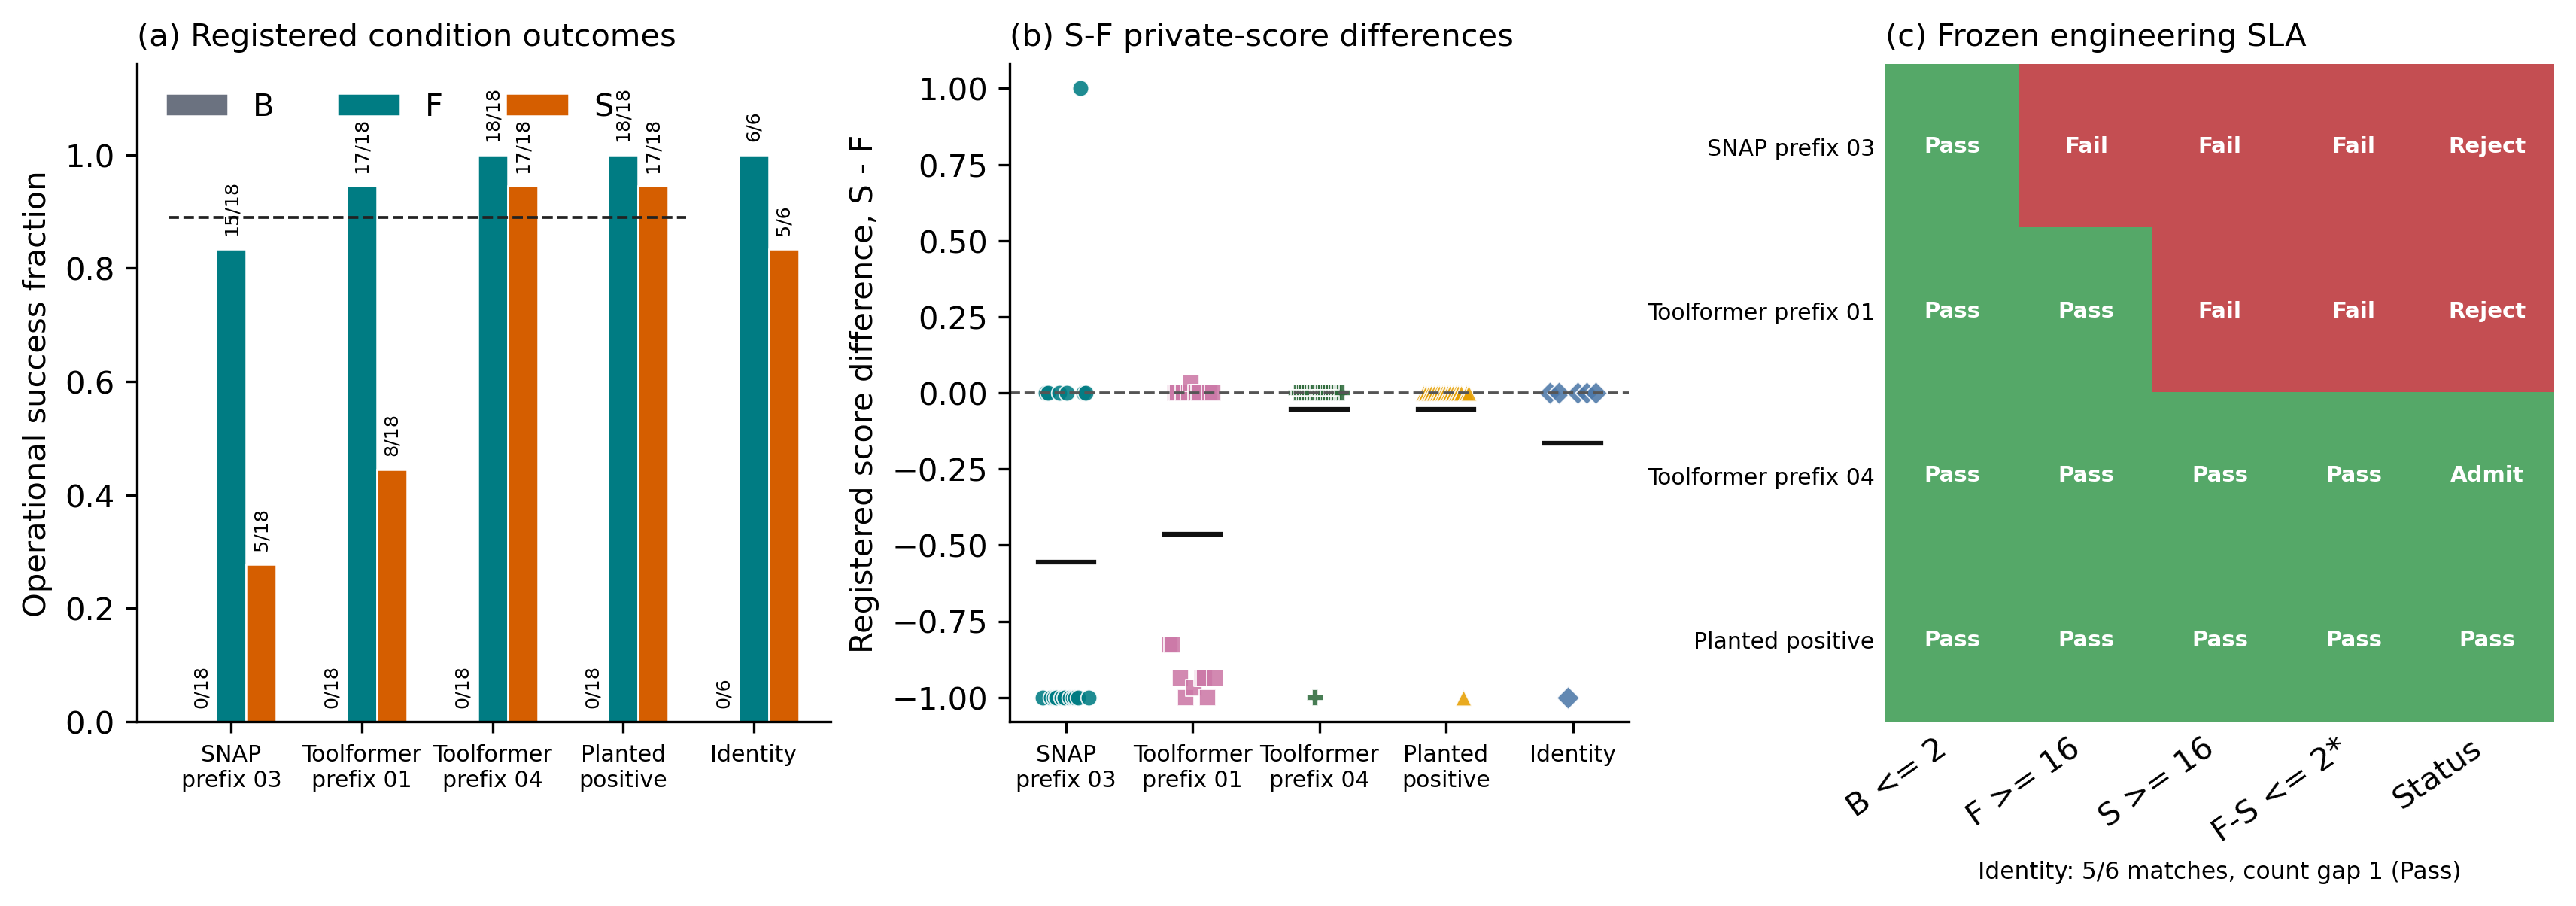
\includegraphics[width=\textwidth]{effectslice_v5_finite_schedule.png}
\caption{Complete V4 evidence plus the separately registered, later V5
candidate.  (a) B/F/S operational successes; labels show exact counts, and the
dashed line marks the 16/18 requirement for the four 18-block strict-subset
families.  (b) Per-block $S-F$ private-score differences; black lines are family
means, not population estimates.  (c) Frozen SLA fields and decisions.  The
starred field is implied by $S\geq16$ at $n=18$; identity uses a separate rule.}
\label{fig:schedules}
\end{figure*}

\begin{table*}[t]
\centering
\small
\setlength{\tabcolsep}{4pt}
\begin{tabular}{lcccccc}
\toprule
Family & Blocks & B success & F success (mean $q$) & S success (mean $q$) & F--S gap & Decision/status \\
\midrule
SNAP real & \SnapRealBlocks & \SnapRealBSuccesses &
\SnapRealFSuccesses\ (\SnapRealFMeanScore) &
\SnapRealSSuccesses\ (\SnapRealSMeanScore) &
\SnapRealFullSliceGap & \SnapRealDecision \\
Toolformer real/negative & \ToolformerRealBlocks & \ToolformerRealBSuccesses &
\ToolformerRealFSuccesses\ (\ToolformerRealFMeanScore) &
\ToolformerRealSSuccesses\ (\ToolformerRealSMeanScore) &
\ToolformerRealFullSliceGap & \ToolformerRealDecision \\
Toolformer prefix 04 & \ToolformerNaturalBlocks & \ToolformerNaturalBSuccesses &
\ToolformerNaturalFSuccesses\ (\ToolformerNaturalFMeanScore) &
\ToolformerNaturalSSuccesses\ (\ToolformerNaturalSMeanScore) &
\ToolformerNaturalFullSliceGap & \ToolformerNaturalDecision \\
Planted positive & \PlantedPositiveBlocks & \PlantedPositiveBSuccesses &
\PlantedPositiveFSuccesses\ (\PlantedPositiveFMeanScore) &
\PlantedPositiveSSuccesses\ (\PlantedPositiveSMeanScore) &
\PlantedPositiveFullSliceGap & \PlantedPositiveDecision \\
Identity instrument & \IdentityControlBlocks & \IdentityControlBSuccesses &
\IdentityControlFSuccesses\ (\IdentityControlFMeanScore) &
\IdentityControlSSuccesses\ (\IdentityControlSMeanScore) &
\IdentityControlFullSliceGap & \IdentityControlDecision \\
\bottomrule
\end{tabular}
\caption{Registered outcomes across sequential V4 and V5 schedules.  Admission
uses the frozen count-level SLA plus complete output and integrity.  The F--S
field is retained but redundant at these thresholds.  Identity is not an
admission and uses its separate 5/6 match rule.}
\label{tab:results}
\end{table*}

\subsection{Three Evidence Questions}

Figure~\ref{fig:schedules} and Table~\ref{tab:results} report both complete
registered schedules.

\paragraph{RQ1: Do B/F/S runs separate two kinds of insufficiency?}
In V4, SNAP B/F/S succeeds in 0/15/5 blocks.  The full artifact misses the
minimum by one, the slice misses it by eleven, and the F--S count gap is ten.
The result therefore finds that neither F nor S meets its frozen sufficiency
requirement for this schedule.

For Toolformer prefix 01, B/F/S succeeds in 0/17/8 blocks.  Here the full
artifact clears its requirement, but the one-atom slice does not and trails F by
nine successes.  The two realized patterns therefore distinguish full-artifact
insufficiency (SNAP) from subset-only insufficiency (Toolformer prefix 01) under
their registered schedules.

\paragraph{RQ2: Do the controls exercise the intended sanity states?}
The planted-positive control is
admitted, this registered negative control is rejected, and byte-identical identity
instrumentation passes despite one fresh-session mismatch.  Thus all three intended
internal sanity states are exercised; they are not estimates of population-level
operating characteristics.

\paragraph{RQ3: Can a post-selected candidate earn a valid local admission on a separately registered, nonoverlapping boundary?}
Prefix 04 existed before V4 but was selected after V4 analysis; V5 then froze
and evaluated it on new private cases.  It retains T01--T04 and omits T05.  B/F/S
succeeds in \ToolformerNaturalBSuccesses{}/\ToolformerNaturalFSuccesses{}/
\ToolformerNaturalSSuccesses{} blocks, with means
\ToolformerNaturalBMeanScore{}/\ToolformerNaturalFMeanScore{}/
\ToolformerNaturalSMeanScore{}.  All six frozen SLA and integrity fields pass, so
the non-planted strict subset is admitted for this task, provider, and private
registry.  The result does not imply that T05 is dispensable for Toolformer in
general; it says this fixed artifact substitutes under the registered V5 boundary.

The omitted atoms offer a plausible diagnosis but not a causal ablation.  SNAP's
slice stops before the matrix-free operator and solver guard; Toolformer prefix
01 stops before every loss and decision unit.  V4 failures are consistent with
those omissions, but no atom-restoration ablation identifies a cause.  Prefix 04
omits only the all-candidate/order unit and passes V5; that is task-local
sufficiency evidence, not a causal or paper-wide redundancy claim.

\subsection{Registered Internal Sanity and Integrity Checks}

The preregistered \texttt{expected\_admission} fields are expectation metadata
only: they encode internal-check expectations for controls and planning
expectations for other candidates.  They never enter the admission decision,
which is recomputed solely from registered outputs and SLA fields.

The planted family removes only redundant T06.  It yields B/F/S counts 0/18/17,
an F--S gap of one, and passes every registered field.  The same scorer and
Toolformer task reject the real one-atom candidate at 0/17/8.  Thus the protocol
does not reject every strict subset, and its registered positive and negative
expectations are both observed.  This is a harness smoke test, not evidence that
a non-planted compact core has been found.  That stronger, still task-local
evidence comes from V5 prefix 04: it was present in the reducer registry before
V4, selected after V4, frozen before V5, and admitted on new private cases.  This
chronology avoids V5 holdout reuse while openly retaining post-V4 selection bias.

For identity instrumentation, F and S are byte-identical yet their fresh
conversations succeed in 6/6 and 5/6 blocks.  Five of six paired success
indicators match and the aggregate gap is one, so the instrument passes.  The
single mismatch is important: artifact identity does not imply trajectory or
patch identity under fresh provider sessions.  This motivates a tolerance-based
finite SLA rather than exact per-pair equality.

Together, planted-positive admission, real-negative rejection, and identity
instrumentation make the registered internal-check status
\VFourCalibrationDecision{} (the macro retains the historical field name).  This
is a task-local sanity and integrity check of the measurement stack, not
sensitivity or specificity over a population of skills.

\subsection{Public Iteration and Evidence Cost}

The two schedules contain \AllProviderConversations{} conversations,
\AllProviderTurns{} provider turns, and \AllActions{} recorded actions.  The
agent requested public tests \AllPublicTestRequests{} times;
\AllPublicTestPasses{} passed and \AllPublicTestFailures{} did not.  V5 alone
contains \VFiveActions{} actions, \VFiveInvalidActions{} invalid actions, one
nonpassing public test, and \VFiveExtraTransportAttempts{} extra transport
attempts.  Every V5 conversation explicitly submitted; all V4 and V5 outputs are
complete.

The provider reported \AllInputTokens{} input and \AllOutputTokens{} output
tokens across \AllTransportAttempts{} transport attempts.  These totals document
evidence cost, not an efficiency advantage.  The protocol deliberately spends
repeated API calls to audit substitution rather than claiming a shorter skill is
cheaper.

\subsection{Analyzer and Release Integrity}

The V4 and V5 bound analyzers stopped before aggregation because a copied check
conflated \texttt{comparison\_role=development\_triage} with the formal
\texttt{evidence\_boundary}.  Narrow post-hoc adapters validate both raw fields,
normalize only that in-memory comparison, and leave preregistrations, runners,
transcripts, patches, scores, thresholds, schedules, and raw manifests unchanged.
Independent outcome/count crosschecks import neither analyzer nor adapter.  They
reread 660 V4 and 198 V5 schema-selected canonical raw-evidence files, verify
terminal private-score and response-ID invariants,
and reproduce every reported count, mean, resource total, control, and decision.
The two archived result-root snapshots contain 1096 files in total.  The canonical selection comprises
block-level \texttt{pair\_manifest.json} and \texttt{run\_report.json}, plus
condition-level \texttt{candidate.patch}, \texttt{run\_result.json}, and
\texttt{transcript.json}; auxiliary duplicate scorer patches and progress/lock
files are excluded.  The canonical post-run manifest records its pre-run roots,
both raw inventories,
analysis lineage, tests, and generated results.  A separate release verifier
enumerates exactly those 858 schema-selected canonical raw-evidence files, requires
set equality with the inventories, and rehashes them plus 24 directly bound
artifacts.  These checks do not
rerun the scorer or independently validate the semantic task contract.

\section{Discussion}

\paragraph{Source-addressed provenance is needed but is not sufficiency.}
A source span can prove that an instruction came from the paper.  It cannot prove
that a selected set contains every operation an agent needs or that the agent will
execute them reliably.  EffectSlice connects provenance to a behavioral record
without conflating them: source atoms answer ``why is this instruction
here?'', while the B/F/S schedule answers ``may this fixed subset substitute for
the complete artifact here?''

\paragraph{The contribution is admission, not compression.}
SkillReducer's self-correcting optimizer can restore content after task failures
\cite{gao2026skillreducer}; Xu and Wu show that representation changes can be
dominated by executor capability \cite{xu2026compression}.  Either pipeline could
feed a candidate into EffectSlice.  Our result does not overturn their aggregate
findings.  It shows that one compact candidate should carry a source identity,
an information-flow boundary, and a local admit/reject record before reuse.

\paragraph{A local admission or rejection is the reusable output.}
For a nonexpert workflow, the useful output need not always be a smaller skill.
If F is not sufficiently reliable, retain the full artifact with a warning.  If F
works but S fails, expose which source units were omitted and do not advertise S
as the paper's core.  If S passes, publish it together with its task, provider,
scorer, schedule, and evidence boundary.  This defines an auditable output
contract; whether it helps people complete real projects faster remains an open
user-study question.

\section{Limitations and Broader Impact}

The study covers two papers, two bounded implementation tasks, one provider
endpoint, one action scaffold, and two sequential registered schedules.  The tasks
exercise paper-specific mechanisms rather than complete SnapATAC2 analyses or
Toolformer training.  The simple prefix candidates are intentionally weak
reducers; we neither run nor claim an official external reducer implementation.
The positive control removes planted redundancy.  Broader candidate generators,
papers, tasks, providers, and independently designed registries are required
before any effectiveness claim.  The one admission among three non-planted
candidates is only a descriptive count across sequential schedules, not a
prospectively registered rate or aggregate performance result.

The atom boundaries, executable instructions, dependency graph, and the claimed
completeness of F were not independently reviewed.  Their digests prove identity,
not semantic correctness.  The two V4 candidates have structurally obvious
omissions.  V5 admits one closer, non-planted Toolformer subset, but it was
selected after V4 and tested on only one new registry for the same task.  This is
not cross-paper or paper-wide equivalence.  Finally, the count-level SLA does not
establish block-level trajectory preservation.

Fresh conversations are not verified independent samples.  The provider exposes
neither a seed nor backend routing guarantees; caching, updates, and shared
infrastructure may induce dependence.  V4 and V5 therefore report only their
complete finite schedules.  Their shared thresholds are fixed engineering
choices, not estimated operating characteristics.  Each decision remains
conditioned on its particular private registry.

The visible public test is intentionally useful and therefore can be overfit.
The terminal private suite limits direct score adaptation but cannot guarantee
semantic generalization beyond its 64 cases.  Independent task-contract review,
additional hidden registries, and adversarial cases would strengthen the record.
The analyzer repairs are fully disclosed and outcome/count cross-checked, but
remain post-registration changes to the analysis path.  V5 repeated the same
role-field defect already found in V4, exposing a regression-testing failure even
though the narrow adapters and crosschecks preserve the reported decisions.
The release supports bit-level audit and offline count recomputation.  It does not
guarantee an end-to-end provider-trajectory rerun: raw pair manifests retain
historical absolute paths, and the provider seed, alias-to-backend mapping, and
backend state are not independently reproducible.  Crosschecks do not rerun the
scorers or independently validate the semantic task contract.

No human participants were studied.  We do not measure understanding, time to
reproduce a paper, or downstream scientific correctness.  Evidence-carrying
admission can reduce overconfident reuse, but a narrow pass can also create false
assurance if its paper, task, provider, and scorer boundaries are omitted.
Generated code remains a supply-chain risk; bounded workspaces and private
scoring reduce but do not eliminate it.

\section{Conclusion}

EffectSlice treats a paper-derived core as a candidate substitution claim.  It
binds source-addressed provenance, visible public development, terminal private
scoring, and registered internal checks into a local decision.  Across
\VFourProviderConversations{} V4
conversations, controls pass, SNAP's registered full artifact misses sufficiency,
and Toolformer prefix 01's slice misses despite sufficient F.  A later schedule
admits non-planted prefix 04 at 0/18/17 B/F/S successes on fresh registered
evidence.  The contribution is a proof-of-concept protocol and evidence package
for an auditable local admit/reject decision, not universal compression.

\bibliography{effectslice_refs}

\end{document}
